\PassOptionsToPackage{unicode=true}{hyperref} % options for packages loaded elsewhere
\PassOptionsToPackage{hyphens}{url}
%
\documentclass[]{article}
\usepackage{lmodern}
\usepackage{amssymb,amsmath}
\usepackage{ifxetex,ifluatex}
\usepackage{fixltx2e} % provides \textsubscript
\ifnum 0\ifxetex 1\fi\ifluatex 1\fi=0 % if pdftex
  \usepackage[T1]{fontenc}
  \usepackage[utf8]{inputenc}
  \usepackage{textcomp} % provides euro and other symbols
\else % if luatex or xelatex
  \usepackage{unicode-math}
  \defaultfontfeatures{Ligatures=TeX,Scale=MatchLowercase}
\fi
% use upquote if available, for straight quotes in verbatim environments
\IfFileExists{upquote.sty}{\usepackage{upquote}}{}
% use microtype if available
\IfFileExists{microtype.sty}{%
\usepackage[]{microtype}
\UseMicrotypeSet[protrusion]{basicmath} % disable protrusion for tt fonts
}{}
\IfFileExists{parskip.sty}{%
\usepackage{parskip}
}{% else
\setlength{\parindent}{0pt}
\setlength{\parskip}{6pt plus 2pt minus 1pt}
}
\usepackage{hyperref}
\hypersetup{
            pdftitle={Algoritma Academy: Programming for Data Science},
            pdfauthor={Samuel Chan},
            pdfborder={0 0 0},
            breaklinks=true}
\urlstyle{same}  % don't use monospace font for urls
\usepackage[margin=1in]{geometry}
\usepackage{color}
\usepackage{fancyvrb}
\newcommand{\VerbBar}{|}
\newcommand{\VERB}{\Verb[commandchars=\\\{\}]}
\DefineVerbatimEnvironment{Highlighting}{Verbatim}{commandchars=\\\{\}}
% Add ',fontsize=\small' for more characters per line
\usepackage{framed}
\definecolor{shadecolor}{RGB}{248,248,248}
\newenvironment{Shaded}{\begin{snugshade}}{\end{snugshade}}
\newcommand{\AlertTok}[1]{\textcolor[rgb]{0.94,0.16,0.16}{#1}}
\newcommand{\AnnotationTok}[1]{\textcolor[rgb]{0.56,0.35,0.01}{\textbf{\textit{#1}}}}
\newcommand{\AttributeTok}[1]{\textcolor[rgb]{0.77,0.63,0.00}{#1}}
\newcommand{\BaseNTok}[1]{\textcolor[rgb]{0.00,0.00,0.81}{#1}}
\newcommand{\BuiltInTok}[1]{#1}
\newcommand{\CharTok}[1]{\textcolor[rgb]{0.31,0.60,0.02}{#1}}
\newcommand{\CommentTok}[1]{\textcolor[rgb]{0.56,0.35,0.01}{\textit{#1}}}
\newcommand{\CommentVarTok}[1]{\textcolor[rgb]{0.56,0.35,0.01}{\textbf{\textit{#1}}}}
\newcommand{\ConstantTok}[1]{\textcolor[rgb]{0.00,0.00,0.00}{#1}}
\newcommand{\ControlFlowTok}[1]{\textcolor[rgb]{0.13,0.29,0.53}{\textbf{#1}}}
\newcommand{\DataTypeTok}[1]{\textcolor[rgb]{0.13,0.29,0.53}{#1}}
\newcommand{\DecValTok}[1]{\textcolor[rgb]{0.00,0.00,0.81}{#1}}
\newcommand{\DocumentationTok}[1]{\textcolor[rgb]{0.56,0.35,0.01}{\textbf{\textit{#1}}}}
\newcommand{\ErrorTok}[1]{\textcolor[rgb]{0.64,0.00,0.00}{\textbf{#1}}}
\newcommand{\ExtensionTok}[1]{#1}
\newcommand{\FloatTok}[1]{\textcolor[rgb]{0.00,0.00,0.81}{#1}}
\newcommand{\FunctionTok}[1]{\textcolor[rgb]{0.00,0.00,0.00}{#1}}
\newcommand{\ImportTok}[1]{#1}
\newcommand{\InformationTok}[1]{\textcolor[rgb]{0.56,0.35,0.01}{\textbf{\textit{#1}}}}
\newcommand{\KeywordTok}[1]{\textcolor[rgb]{0.13,0.29,0.53}{\textbf{#1}}}
\newcommand{\NormalTok}[1]{#1}
\newcommand{\OperatorTok}[1]{\textcolor[rgb]{0.81,0.36,0.00}{\textbf{#1}}}
\newcommand{\OtherTok}[1]{\textcolor[rgb]{0.56,0.35,0.01}{#1}}
\newcommand{\PreprocessorTok}[1]{\textcolor[rgb]{0.56,0.35,0.01}{\textit{#1}}}
\newcommand{\RegionMarkerTok}[1]{#1}
\newcommand{\SpecialCharTok}[1]{\textcolor[rgb]{0.00,0.00,0.00}{#1}}
\newcommand{\SpecialStringTok}[1]{\textcolor[rgb]{0.31,0.60,0.02}{#1}}
\newcommand{\StringTok}[1]{\textcolor[rgb]{0.31,0.60,0.02}{#1}}
\newcommand{\VariableTok}[1]{\textcolor[rgb]{0.00,0.00,0.00}{#1}}
\newcommand{\VerbatimStringTok}[1]{\textcolor[rgb]{0.31,0.60,0.02}{#1}}
\newcommand{\WarningTok}[1]{\textcolor[rgb]{0.56,0.35,0.01}{\textbf{\textit{#1}}}}
\usepackage{graphicx,grffile}
\makeatletter
\def\maxwidth{\ifdim\Gin@nat@width>\linewidth\linewidth\else\Gin@nat@width\fi}
\def\maxheight{\ifdim\Gin@nat@height>\textheight\textheight\else\Gin@nat@height\fi}
\makeatother
% Scale images if necessary, so that they will not overflow the page
% margins by default, and it is still possible to overwrite the defaults
% using explicit options in \includegraphics[width, height, ...]{}
\setkeys{Gin}{width=\maxwidth,height=\maxheight,keepaspectratio}
\setlength{\emergencystretch}{3em}  % prevent overfull lines
\providecommand{\tightlist}{%
  \setlength{\itemsep}{0pt}\setlength{\parskip}{0pt}}
\setcounter{secnumdepth}{0}
% Redefines (sub)paragraphs to behave more like sections
\ifx\paragraph\undefined\else
\let\oldparagraph\paragraph
\renewcommand{\paragraph}[1]{\oldparagraph{#1}\mbox{}}
\fi
\ifx\subparagraph\undefined\else
\let\oldsubparagraph\subparagraph
\renewcommand{\subparagraph}[1]{\oldsubparagraph{#1}\mbox{}}
\fi

% set default figure placement to htbp
\makeatletter
\def\fps@figure{htbp}
\makeatother


\title{Algoritma Academy: Programming for Data Science}
\author{Samuel Chan}
\date{20 August, 2020}

\begin{document}
\maketitle

Before you go ahead and run the code in this coursebook, it's often a
good idea to go through some initial setup. Under the \emph{Libraries
and Setup} tab you'll see some code to initialize our workspace, and the
libraries we'll be using for the projects. You may want to make sure
that the libraries are installed beforehand by referring back to the
packages listed here. Under the \emph{Training Focus} tab we'll outline
the syllabus, identify the key objectives and set up expectations for
each module.

\hypertarget{background}{%
\section{Background}\label{background}}

\hypertarget{algoritma}{%
\subsection{Algoritma}\label{algoritma}}

The following coursebook is produced by the team at
\href{https://algorit.ma}{Algoritma} for its Data Science Academy
workshops. The coursebook is intended for a restricted audience only,
i.e.~the individuals and organizations having received this coursebook
directly from the training organization. It may not be reproduced,
distributed, translated or adapted in any form outside these individuals
and organizations without permission.

Algoritma is a data science education center with bootcamp programs
offered in:

\begin{itemize}
\tightlist
\item
  Bahasa Indonesia (Jakarta campus)\\
\item
  English (Singapore campus)
\end{itemize}

\hypertarget{lifelong-learning-benefits}{%
\subsubsection{Lifelong Learning
Benefits}\label{lifelong-learning-benefits}}

If you're an active student or an alumni member, you also qualify for
all our future workshops, 100\% free of charge as part of your
\textbf{lifelong learning benefits}. It is a new initiative to help you
gain mastery and advance your knowledge in the field of data
visualization, machine learning, computer vision, natural language
processing (NLP) and other sub-fields of data science. All workshops
conducted by us (from 1-day to 5-day series) are available to you
free-of-charge, and the benefits \textbf{never expire}.

\hypertarget{second-edition}{%
\subsubsection{Second Edition}\label{second-edition}}

This coursebook is initially written in 2017.

This is the second edition, written in late August 2020. Some of the
code has been refactored to work with the latest major version of R,
version 4.0. I would like to thank the incredible instructor team at
Algoritma for their thorough input and assistance in the authoring and
reviewing process.

\hypertarget{libraries-and-setup}{%
\subsection{Libraries and Setup}\label{libraries-and-setup}}

We'll set-up caching for this notebook given how computationally
expensive some of the code we will write can get.

\begin{Shaded}
\begin{Highlighting}[]
\CommentTok{# chunk set up}
\NormalTok{knitr}\OperatorTok{::}\NormalTok{opts_chunk}\OperatorTok{$}\KeywordTok{set}\NormalTok{(}\DataTypeTok{cache=}\OtherTok{TRUE}\NormalTok{,}
                      \DataTypeTok{fig.align =} \StringTok{"center"}\NormalTok{,}
                      \DataTypeTok{comment =} \StringTok{"#>"}
\NormalTok{                      )}

\CommentTok{# set up scientific notation}
\KeywordTok{options}\NormalTok{(}\DataTypeTok{scipen =} \DecValTok{9999}\NormalTok{)}

\CommentTok{# clear Global Environment}
\KeywordTok{rm}\NormalTok{(}\DataTypeTok{list=}\KeywordTok{ls}\NormalTok{())}
\end{Highlighting}
\end{Shaded}

You will need to use \texttt{install.packages()} to install any packages
that are not already downloaded onto your machine. You then load the
package into your workspace using the \texttt{library()} function:

\begin{Shaded}
\begin{Highlighting}[]
\KeywordTok{library}\NormalTok{(dplyr)}
\KeywordTok{library}\NormalTok{(skimr)}
\end{Highlighting}
\end{Shaded}

\hypertarget{training-objectives}{%
\subsection{Training Objectives}\label{training-objectives}}

The primary objective of this course is to provide a comprehensive
introduction to the science of statistical programming and the toolsets
required to succeed with data science work. The syllabus covers:

\begin{itemize}
\item
  \textbf{Basic Programming in R}
\item
  Objects and Environment
\item
  Data Classes in R
\item
  Data Structures in R\\
\item
  Data Science Workflow
\item
  R Scripts and R Markdown
\item
  \textbf{Data Manipulation}\\
\item
  Read \& Extracting Data\\
\item
  Practical Data Cleansing\\
\item
  Data Transformation
\item
  \textbf{Statistical Computing}\\
\item
  Organizing your Project\\
\item
  Modern Tools for Data Analysis\\
\item
  Reproducible Data Science
\end{itemize}

\begin{center}\rule{0.5\linewidth}{0.5pt}\end{center}

By the end of the workshop, Academy students can choose to complete
either of the Learn-By-Building modules as their graded assignment:

\textbf{R Script to clean \& transform the data}\\
A programming script that perform various data cleansing tasks and
output the result in an appropriate format for further data science
work.

\textbf{Reproducible Data Science}\\
Create an R Markdown file that combines data transformation code with
explanatory text. Add formatting styles and hierarchical structure using
Markdown.

\hypertarget{r-programming}{%
\section{R Programming}\label{r-programming}}

Since you'll spend a great deal of your time working with data in R and
RStudio, I think it's important to get yourself very familiar with this
IDE (Integrated Development Environment). RStudio is the most popular
integrated development for R and is a core tool for data science teams
in Airbnb\footnote{\href{https://peerj.com/preprints/3182.pdf}{How R
  Helps AirBnB make the most of its data}}, Uber\footnote{\href{https://eng.uber.com/tech-stack-part-one/}{Uber
  Engineering's Tech Stack: The Foundation}} etc., and is a tool we'll
be using throughout the Academy workshops.

If you're a seasoned programmer, the \textbf{Option + Shift + K} (Alt +
Shift + K on Windows) combination will bring up a shortcut reference
guide that helps you use RStudio more effectively.

\hypertarget{why-learn-r-at-all}{%
\subsection{Why learn R at all?}\label{why-learn-r-at-all}}

\begin{enumerate}
\def\labelenumi{\arabic{enumi}.}
\item
  \textbf{Built by statisticians, for statisticians.}\\
  R is a statistical programming language created by Ross Ihaka and
  Robert Gentleman at the Department of Statistics, at the University of
  Auckland (New Zealand). R is created for the purpose of data analysis
  and as such, is different in nature from traditional programming
  languages. R is not just a statistical programming language, it is a
  complete environment for data scientist and the most widely used data
  analysis software today\footnote{\href{http://mran.revolutionanalytics.com/rro/}{Microsoft
    R Open: The Enhanced R Distribution}}.
\item
  \textbf{Libraries.}\\
  R's libraries extend R's graphical abilities, and adds out-of-the-box
  functionalities for linear and non-linear modeling, statistical tests
  (confidence tests, P-value, t-test etc), time-series analysis, and
  various machine learning tools such as regression algorithms,
  classification algorithms, and clustering algorithms. The R community
  is noted for its active contributions in terms of packages and boasts
  nearly 20,000 packages to date.
\item
  \textbf{Open Source.} Part of the reason for its active and rapidly
  growing community is the open-source nature of R. Users can contribute
  packages -- many of which packaged some of the most advanced
  statistical tools that are not found in other commercial, proprietary
  statistical computing softwares.
\item
  \textbf{Used by the biggest software companies in the world.}\\
  R is used by Google to calculate ROI on advertising campaigns and
  estimate causal effect (say, estimate the impact of an app feature on
  app downloads or number of additional sales from an AdWords campaign);
  In fact, it even released its own R packages to allow other R users to
  do similar analysis using the same tool\footnote{\href{https://opensource.googleblog.com/2014/09/causalimpact-new-open-source-package.html}{CausalImpact:
    A new open-source package for estimating causal effects in time
    series}}. Data Science employees at Google participate in User
  Groups to discuss how R is used in Google (answer: it's used very
  widely in a production environment at Google and Google integrates R
  with many of their own technologies), publishing
  \href{https://code.google.com/archive/p/google-prediction-api-r-client/}{its
  own R client for the Google Prediction API},
  \href{http://web.stanford.edu/class/cs109l/unrestricted/resources/google-style.html}{Google's
  R style guide}, and its developers have released a number of R
  packages over the years. Microsoft first uses R for Azure capacity
  planning, Xbox's TrueSkill Matchmaking System, player churn analysis,
  in-game purchase optimization, fraud detection, and other internal
  services across Microsoft's line of products\footnote{\href{http://blog.revolutionanalytics.com/2015/06/r-at-microsoft.html}{R
    at Microsoft}}, and then went on to acquire Revolution Analytics,
  whom products were then rebranded and renewed by Microsoft and now
  known as Microsoft R Server, Microsoft R Open, Microsoft Data Science
  Virtual Machine etc.
\item
  \textbf{Ready for big data}\\
  RHadoop, ParallelR, Revolution R Enterprise and a handful of other
  toolkits adds powerful big data support, allowing data engineers to
  create custom parallel and distributed algorithms to handle parallel /
  map-reduce programming in R. This makes R a popular choice for big
  data analytics and high performance, enterprise-level analytics
  platform.
\item
  \textbf{Employability!}\\
  R is a required skill for data science roles across all top
  Indonesian's startups: GoJek, Traveloka, Uber, Shopee, Twitter,
  HappyFresh etc. Do a quick search on job portals (Tech In Asia's Jobs,
  JobStreet etc) and you'll see R is a highly sought-after language
  skill.
\end{enumerate}

The \href{Google's\%20R\%20Style\%20Guide}{Google's R Style Guide} is
the one we'll adhere to - if this is the first time you're writing R
code, I recommend you adopt these ``best practices'' as a certain level
of strictness can make you a more disciplined and methodical programmer
in the long run.

\hypertarget{r-programming-basics}{%
\subsection{R Programming Basics}\label{r-programming-basics}}

It pays to get yourself familiar with R and RStudio, the IDE
(interactive development environment). In our workshop, we'll discuss in
more details the various functionalities of RStudio's interface, and if
this is the first time you're working in a code environment, spend some
time to get yourself familiar with this IDE along with the RMarkdown
format as you'll be working with it a lot!

Before moving forward, make sure you have a solid understanding of the
following:

\begin{itemize}
\tightlist
\item
  R as a statistical programming language\\
\item
  RStudio as a code editor and integrated development environment
\item
  The RMarkdown format
\end{itemize}

To get started, let's write our first R code by typing \texttt{getwd()}
into the Console (bottom of the screen), or by running in from within a
Chunk (look for the green ``run'' button):

\begin{Shaded}
\begin{Highlighting}[]
\CommentTok{# This is a comment}
\KeywordTok{getwd}\NormalTok{()}
\end{Highlighting}
\end{Shaded}

\begin{verbatim}
#> [1] "/Users/samuel/Downloads/[Algoritma] _ Data Science Academy /[Algoritma] 1 Data Science Academy _ Programming for Data Science/P4DS"
\end{verbatim}

\begin{Shaded}
\begin{Highlighting}[]
\CommentTok{# setwd(...)}
\end{Highlighting}
\end{Shaded}

Notice the ``\#'' character in the first and third line of the code
chunk, indicating to R that it's a comment and should be ignored.
\texttt{setwd()} was ignored because it's on the same line and to the
right of the ``\#'' character. As you may have expected,
\texttt{setwd()} is used to change our working directory by setting a
new one.

R is \textbf{case-sensitive} so ``Algoritma'' and ``algoritma'' are
different symbols and will point to different variables.

\begin{Shaded}
\begin{Highlighting}[]
\NormalTok{activity <-}\StringTok{ "Programming"}
\NormalTok{activity }\OperatorTok{==}\StringTok{ "programming"}
\end{Highlighting}
\end{Shaded}

\begin{verbatim}
#> [1] FALSE
\end{verbatim}

\begin{Shaded}
\begin{Highlighting}[]
\KeywordTok{print}\NormalTok{(}\KeywordTok{paste}\NormalTok{(activity, }\StringTok{"in data science."}\NormalTok{))}
\end{Highlighting}
\end{Shaded}

\begin{verbatim}
#> [1] "Programming in data science."
\end{verbatim}

\begin{Shaded}
\begin{Highlighting}[]
\CommentTok{# Un-comment the following line; Observe that object 'Activity' don't exist!}
\CommentTok{# print(Activity) will not work}
\end{Highlighting}
\end{Shaded}

\hypertarget{vectors}{%
\subsubsection{Vectors}\label{vectors}}

Speaking of objects, some of the most common data types that you'll come
across are: - character\\
- numeric\\
- integer\\
- logical

The most basic form of an R object is a vector. As a rule, a vector can
only contain objects of the same class:

\begin{Shaded}
\begin{Highlighting}[]
\NormalTok{vector1 <-}\StringTok{ }\KeywordTok{c}\NormalTok{(}\StringTok{"learning"}\NormalTok{, }\StringTok{"data"}\NormalTok{, }\StringTok{"science"}\NormalTok{, }\DecValTok{2018}\NormalTok{)}
\KeywordTok{class}\NormalTok{(vector1)}
\end{Highlighting}
\end{Shaded}

\begin{verbatim}
#> [1] "character"
\end{verbatim}

\begin{Shaded}
\begin{Highlighting}[]
\NormalTok{vector2 <-}\StringTok{ }\KeywordTok{c}\NormalTok{(}\DecValTok{1}\NormalTok{, }\OtherTok{FALSE}\NormalTok{, }\OtherTok{FALSE}\NormalTok{, }\DecValTok{0}\NormalTok{)}
\KeywordTok{class}\NormalTok{(vector2)}
\end{Highlighting}
\end{Shaded}

\begin{verbatim}
#> [1] "numeric"
\end{verbatim}

Also observe how we use the \texttt{c()} function to concatenate objects
together to form a vector.

\texttt{vector1} is now an object in our global environment, but if
you're paying attention, you'll notice that it is a \textbf{character
vector}. While 2018 itself is a numeric, because of the ``same-class''
rule we learn above, 2018 was coerced into a character so that the
resulting vector is valid. 2018 (the numeric) is ``2018'' (character) as
a result:

\begin{Shaded}
\begin{Highlighting}[]
\NormalTok{vector1}
\end{Highlighting}
\end{Shaded}

\begin{verbatim}
#> [1] "learning" "data"     "science"  "2018"
\end{verbatim}

Similarly, in \texttt{vector2}, \texttt{1} is a numeric, and
\texttt{FALSE} is a logical, and therefore the \texttt{FALSE} values are
coerced into a numeric. Go ahead and print out \texttt{vector2} as a
confirmation:

\begin{Shaded}
\begin{Highlighting}[]
\CommentTok{# your code here:}
\end{Highlighting}
\end{Shaded}

R objects may have attributes like \texttt{names}, \texttt{class},
\texttt{length}, \texttt{colnames}, \texttt{dim} etc:

\begin{Shaded}
\begin{Highlighting}[]
\KeywordTok{names}\NormalTok{(vector2) <-}\StringTok{ }\KeywordTok{c}\NormalTok{(}\StringTok{"User ID"}\NormalTok{, }\StringTok{"Active"}\NormalTok{, }\StringTok{"Cart Items"}\NormalTok{, }\StringTok{"Payment"}\NormalTok{)}
\KeywordTok{length}\NormalTok{(vector2)}
\end{Highlighting}
\end{Shaded}

\begin{verbatim}
#> [1] 4
\end{verbatim}

\begin{Shaded}
\begin{Highlighting}[]
\NormalTok{vector2}
\end{Highlighting}
\end{Shaded}

\begin{verbatim}
#>    User ID     Active Cart Items    Payment 
#>          1          0          0          0
\end{verbatim}

Recall how implicit coercion (R's default) takes place earlier when we
create our \texttt{vector1} and \texttt{vector2}. We could explicitly
coerce one class to another:

\begin{Shaded}
\begin{Highlighting}[]
\NormalTok{vector2 <-}\StringTok{ }\KeywordTok{c}\NormalTok{(}\DecValTok{1}\NormalTok{,}\OtherTok{FALSE}\NormalTok{,}\OtherTok{FALSE}\NormalTok{,}\DecValTok{0}\NormalTok{)}
\NormalTok{vector2.b <-}\StringTok{ }\KeywordTok{as.logical}\NormalTok{(vector2)}
\NormalTok{vector2.b}
\end{Highlighting}
\end{Shaded}

\begin{verbatim}
#> [1]  TRUE FALSE FALSE FALSE
\end{verbatim}

\begin{Shaded}
\begin{Highlighting}[]
\KeywordTok{class}\NormalTok{(vector2.b)}
\end{Highlighting}
\end{Shaded}

\begin{verbatim}
#> [1] "logical"
\end{verbatim}

\textbf{Dive Deeper:}

Create a vector and name it \texttt{customers}. Store 4 names in the
vector and make sure it is a \texttt{character} vector. Create another
vector and name it \texttt{age}, store 4 numeric in the vector and make
sure it is a \texttt{numeric} vector.

\begin{Shaded}
\begin{Highlighting}[]
\CommentTok{# Your code here:}
\end{Highlighting}
\end{Shaded}

\begin{enumerate}
\def\labelenumi{\arabic{enumi}.}
\setcounter{enumi}{1}
\tightlist
\item
  Use \texttt{class()} and \texttt{length()} in the code chunk below to
  verify that you have done the exercise above correctly:
\end{enumerate}

\begin{Shaded}
\begin{Highlighting}[]
\CommentTok{# Your code here:}
\end{Highlighting}
\end{Shaded}

\begin{enumerate}
\def\labelenumi{\arabic{enumi}.}
\setcounter{enumi}{2}
\tightlist
\item
  Create another vector and name it \texttt{suppliers}. Store 3 names in
  it:
\end{enumerate}

\begin{Shaded}
\begin{Highlighting}[]
\CommentTok{# Your code here}
\end{Highlighting}
\end{Shaded}

\begin{enumerate}
\def\labelenumi{\arabic{enumi}.}
\setcounter{enumi}{3}
\tightlist
\item
  Join the \texttt{customers} and \texttt{suppliers} vector into one
  vector using the concatenate technique you've learned, which is
  \texttt{c()}.
\end{enumerate}

\begin{Shaded}
\begin{Highlighting}[]
\CommentTok{# Your code here:}
\end{Highlighting}
\end{Shaded}

If you've managed to execute the above exercises in the dive deeper
section: congratulations! Throughout the course you'll do a number of
these exercises, and they are useful revision tools that you should take
advantage of to test your knowledge and make sure you have a full grasp
of the topics being assessed.

You've see how numeric and character classes and even made a few vectors
of your own above! But R has other object types and we'll take a look at
them:

\begin{Shaded}
\begin{Highlighting}[]
\CommentTok{# character}
\NormalTok{tempo <-}\StringTok{ }\KeywordTok{c}\NormalTok{(}\StringTok{"Algoritma"}\NormalTok{, }\StringTok{"Indonesia"}\NormalTok{, }\StringTok{"e-Commerce"}\NormalTok{, }\StringTok{"Jakarta"}\NormalTok{)}
\CommentTok{# numeric}
\NormalTok{tempo <-}\StringTok{ }\KeywordTok{c}\NormalTok{(}\OperatorTok{-}\DecValTok{1}\NormalTok{, }\DecValTok{1}\NormalTok{, }\DecValTok{2}\NormalTok{, }\DecValTok{3}\OperatorTok{/}\DecValTok{4}\NormalTok{, }\FloatTok{0.5}\NormalTok{)}
\CommentTok{# integer}
\NormalTok{tempo <-}\StringTok{ }\KeywordTok{c}\NormalTok{(1L, 2L)}
\CommentTok{# integer}
\NormalTok{tempo <-}\StringTok{ }\DecValTok{5}\OperatorTok{:}\DecValTok{8}
\CommentTok{# logical}
\NormalTok{tempo <-}\StringTok{ }\KeywordTok{c}\NormalTok{(}\OtherTok{TRUE}\NormalTok{, }\OtherTok{TRUE}\NormalTok{, }\OtherTok{FALSE}\NormalTok{)}
\end{Highlighting}
\end{Shaded}

A quick note on integers: they cannot take decimal or fractional values,
while numerics can. Numerics act more like the ``float'' or ``double''
types supported by many other programming languages.

\hypertarget{matrix}{%
\subsubsection{Matrix}\label{matrix}}

When we create a vector and give it a dimension attribute, we end up
with a matrix:

\begin{Shaded}
\begin{Highlighting}[]
\NormalTok{matri <-}\StringTok{ }\KeywordTok{matrix}\NormalTok{(}\DecValTok{11}\OperatorTok{:}\DecValTok{16}\NormalTok{, }\DataTypeTok{nrow=}\DecValTok{3}\NormalTok{, }\DataTypeTok{ncol=}\DecValTok{2}\NormalTok{)}
\KeywordTok{dim}\NormalTok{(matri)}
\end{Highlighting}
\end{Shaded}

\begin{verbatim}
#> [1] 3 2
\end{verbatim}

\begin{Shaded}
\begin{Highlighting}[]
\NormalTok{matri}
\end{Highlighting}
\end{Shaded}

\begin{verbatim}
#>      [,1] [,2]
#> [1,]   11   14
#> [2,]   12   15
#> [3,]   13   16
\end{verbatim}

Notice how the values fill up by column from the {[}1,1{]} position,
which is the most upper-left position.

Once created, we can refer to any row or column using R's subsetting
operator:

\begin{Shaded}
\begin{Highlighting}[]
\NormalTok{matri[}\DecValTok{1}\NormalTok{,]}
\end{Highlighting}
\end{Shaded}

\begin{verbatim}
#> [1] 11 14
\end{verbatim}

\begin{Shaded}
\begin{Highlighting}[]
\NormalTok{matri[,}\DecValTok{2}\NormalTok{]}
\end{Highlighting}
\end{Shaded}

\begin{verbatim}
#> [1] 14 15 16
\end{verbatim}

We could also have constructed a matrix by giving an existing vector the
\texttt{dim} attribute:

\begin{Shaded}
\begin{Highlighting}[]
\NormalTok{numbers <-}\StringTok{ }\DecValTok{11}\OperatorTok{:}\DecValTok{16}
\KeywordTok{dim}\NormalTok{(numbers) <-}\StringTok{ }\KeywordTok{c}\NormalTok{(}\DecValTok{2}\NormalTok{,}\DecValTok{3}\NormalTok{)}
\NormalTok{numbers}
\end{Highlighting}
\end{Shaded}

\begin{verbatim}
#>      [,1] [,2] [,3]
#> [1,]   11   13   15
#> [2,]   12   14   16
\end{verbatim}

Notice \texttt{c(2,3)} means ``2 rows, 3 columns''. Contrast this to our
\texttt{matri} object above and the way we constructed matrices using
two different approach.

Another interesting way to construct a matrix:

\begin{Shaded}
\begin{Highlighting}[]
\NormalTok{accounts <-}\StringTok{ }\KeywordTok{c}\NormalTok{(}\StringTok{"AlphaMall"}\NormalTok{, }\StringTok{"BetaMall"}\NormalTok{, }\StringTok{"OmegaMall"}\NormalTok{)}
\NormalTok{sales <-}\StringTok{ }\KeywordTok{c}\NormalTok{(}\DecValTok{400}\NormalTok{,}\DecValTok{320}\NormalTok{,}\DecValTok{380}\NormalTok{)}
\NormalTok{returns <-}\StringTok{ }\KeywordTok{c}\NormalTok{(}\DecValTok{0}\NormalTok{,}\DecValTok{0}\NormalTok{,}\DecValTok{480}\NormalTok{)}
\NormalTok{netsales <-}\StringTok{ }\NormalTok{sales }\OperatorTok{-}\StringTok{ }\NormalTok{returns}
\CommentTok{# cbind = bind as columns}
\CommentTok{# rbind = bind as rows}
\CommentTok{# rbind(accounts, sales, returns)}

\NormalTok{sales_records <-}\StringTok{ }\KeywordTok{cbind}\NormalTok{(accounts, sales, netsales)}
\end{Highlighting}
\end{Shaded}

\texttt{sales\_record} is now a matrix. Go ahead and print it, then
observe how 400 (numeric) has been coerced into ``400'' (strings) so the
resulting matrix is a valid R object.

\textbf{Dive Deeper:}\\
1. You learned how to bind the three vectors by columns. Now create a
matrix named \texttt{sales\_records} and bind \texttt{sales},
\texttt{returns} and \texttt{netsales} by rows (instead of columns). You
can do this with \texttt{rbind} (row-bind)

\begin{Shaded}
\begin{Highlighting}[]
\CommentTok{# Your code here}
\end{Highlighting}
\end{Shaded}

\begin{enumerate}
\def\labelenumi{\arabic{enumi}.}
\setcounter{enumi}{1}
\tightlist
\item
  You can optionally check that you've done the above step correctly by
  printing out the matrix and / or use \texttt{dim()} to verify that is
  in fact a 3x3 matrix. Now assign \texttt{accounts} as column names to
  your matrix. To assign column names to a matrix, we can use
  \texttt{colnames(mymatrix)\ \textless{}-\ c("Name1",\ "Name2",\ "Name3")}:
\end{enumerate}

\begin{Shaded}
\begin{Highlighting}[]
\CommentTok{# Your code here}
\end{Highlighting}
\end{Shaded}

\begin{enumerate}
\def\labelenumi{\arabic{enumi}.}
\setcounter{enumi}{2}
\tightlist
\item
  Print our \texttt{sales\_records}:
\end{enumerate}

\begin{Shaded}
\begin{Highlighting}[]
\CommentTok{# Your code here}
\end{Highlighting}
\end{Shaded}

\textbf{Dive Deeper}

Recall that I've repeatedly stressed that as a rule, a vector can
contain objects of the same class? Consider the following code:

\begin{itemize}
\item
  \begin{enumerate}
  \def\labelenumi{\arabic{enumi}.}
  \tightlist
  \item
    What is the class of the resulting vector \texttt{quiz1}?
  \end{enumerate}
\item
  \begin{enumerate}
  \def\labelenumi{\arabic{enumi}.}
  \setcounter{enumi}{1}
  \tightlist
  \item
    What is the dimensions attribute of \texttt{quiz1}?\\
  \end{enumerate}
\item
  \begin{enumerate}
  \def\labelenumi{\arabic{enumi}.}
  \setcounter{enumi}{2}
  \tightlist
  \item
    How many times did implicit coercion happened?
  \end{enumerate}
\end{itemize}

\hypertarget{list}{%
\subsubsection{List}\label{list}}

There is a type of R object that is exempted from the rule we repeatedly
mention above, and it's the \textbf{List}:

\begin{Shaded}
\begin{Highlighting}[]
\NormalTok{our.list <-}\StringTok{ }\KeywordTok{list}\NormalTok{(}\OtherTok{TRUE}\NormalTok{, }\StringTok{"TRUE"}\NormalTok{, }\KeywordTok{c}\NormalTok{(}\DecValTok{1}\NormalTok{,}\DecValTok{6}\NormalTok{,}\DecValTok{12}\NormalTok{), }\DecValTok{1}\OperatorTok{+}\NormalTok{5i)}
\NormalTok{our.list}
\end{Highlighting}
\end{Shaded}

\begin{verbatim}
#> [[1]]
#> [1] TRUE
#> 
#> [[2]]
#> [1] "TRUE"
#> 
#> [[3]]
#> [1]  1  6 12
#> 
#> [[4]]
#> [1] 1+5i
\end{verbatim}

A list, as we've observed above, can contain elements that are of
different classes from other members of the list. You can can subset
from a list much like how you've done earlier: however, any subsets
using a single square bracket \texttt{{[}{]}} will return a list. To
return the elements itself, use double square-brackets:
\texttt{{[}{[}{]}{]}}

Demonstration of subsetting elements from our list:

\begin{Shaded}
\begin{Highlighting}[]
\NormalTok{our.list[}\DecValTok{3}\NormalTok{]}
\end{Highlighting}
\end{Shaded}

\begin{verbatim}
#> [[1]]
#> [1]  1  6 12
\end{verbatim}

\begin{Shaded}
\begin{Highlighting}[]
\NormalTok{our.list[[}\DecValTok{3}\NormalTok{]]}
\end{Highlighting}
\end{Shaded}

\begin{verbatim}
#> [1]  1  6 12
\end{verbatim}

\begin{Shaded}
\begin{Highlighting}[]
\KeywordTok{class}\NormalTok{(our.list[}\DecValTok{3}\NormalTok{])}
\end{Highlighting}
\end{Shaded}

\begin{verbatim}
#> [1] "list"
\end{verbatim}

\begin{Shaded}
\begin{Highlighting}[]
\KeywordTok{class}\NormalTok{(our.list[[}\DecValTok{3}\NormalTok{]])}
\end{Highlighting}
\end{Shaded}

\begin{verbatim}
#> [1] "numeric"
\end{verbatim}

\hypertarget{factors}{%
\subsubsection{Factors}\label{factors}}

Another important concept in R is factors - many statistical modeling
techniques and prediction algorithms treat factors specially either as a
target outcome (in machine learning language) or dependent variable (in
statistics) while many other modeling techniques treat factors specially
when they're used as independent variables. Factors is useful in
representing categorical variables whether or not they are unordered
(cash, credit, transfer) or ordered (high volume, normal volume, low
volume):

\begin{Shaded}
\begin{Highlighting}[]
\NormalTok{categories <-}\StringTok{ }\KeywordTok{factor}\NormalTok{(}\KeywordTok{c}\NormalTok{(}\StringTok{"OfficeSupplies"}\NormalTok{, }\StringTok{"Computers"}\NormalTok{, }\StringTok{"Packaging"}\NormalTok{, }\StringTok{"Machinery"}\NormalTok{, }\StringTok{"Building"}\NormalTok{))}
\NormalTok{categories }\CommentTok{# levels are sorted alphabetically unless through the levels argument}
\end{Highlighting}
\end{Shaded}

\begin{verbatim}
#> [1] OfficeSupplies Computers      Packaging      Machinery      Building      
#> Levels: Building Computers Machinery OfficeSupplies Packaging
\end{verbatim}

\hypertarget{data-frames}{%
\subsubsection{Data Frames}\label{data-frames}}

Data frames can be thought of as a special case of lists where every
element of the list has to have the same length. Each element of the
list can be thought of as a column in the data frame.

\begin{Shaded}
\begin{Highlighting}[]
\NormalTok{categories_df <-}\StringTok{ }\KeywordTok{data.frame}\NormalTok{(}\DataTypeTok{categories=}\KeywordTok{c}\NormalTok{(}\StringTok{"OfficeSupplies"}\NormalTok{, }\StringTok{"Computers"}\NormalTok{, }\StringTok{"Packaging"}\NormalTok{, }\StringTok{"Machinery"}\NormalTok{, }\StringTok{"Building"}\NormalTok{), }\DataTypeTok{category_id=}\DecValTok{111}\OperatorTok{:}\DecValTok{115}\NormalTok{)}
\NormalTok{categories_df}
\end{Highlighting}
\end{Shaded}

\begin{verbatim}
#>       categories category_id
#> 1 OfficeSupplies         111
#> 2      Computers         112
#> 3      Packaging         113
#> 4      Machinery         114
#> 5       Building         115
\end{verbatim}

And we can perform mathematical operations on our dataframes, the same
way we can do it with matrices. If we need to update our system by
adding one new category on the top of the list such that all existing
IDs are incremented by one, we can do so:

\begin{Shaded}
\begin{Highlighting}[]
\NormalTok{categories_df}\OperatorTok{$}\NormalTok{category_id }\OperatorTok{+}\StringTok{ }\DecValTok{1}
\end{Highlighting}
\end{Shaded}

\begin{verbatim}
#> [1] 112 113 114 115 116
\end{verbatim}

Notice that here we're accessing the \texttt{category\_id} column using
the `\$' operator.

Hopefully by now you also observe how R conveniently applies implicit
coercion so our data frame and matrix can be multiplied. This is another
nice property of R!

\begin{Shaded}
\begin{Highlighting}[]
\KeywordTok{class}\NormalTok{(}\DecValTok{1}\OperatorTok{-}\OtherTok{TRUE}\NormalTok{)}
\end{Highlighting}
\end{Shaded}

\begin{verbatim}
#> [1] "numeric"
\end{verbatim}

\begin{Shaded}
\begin{Highlighting}[]
\OtherTok{TRUE} \OperatorTok{+}\StringTok{ }\OtherTok{TRUE} \OperatorTok{*}\StringTok{ }\DecValTok{34}
\end{Highlighting}
\end{Shaded}

\begin{verbatim}
#> [1] 35
\end{verbatim}

\hypertarget{r-programming-with-retail}{%
\section{R Programming with Retail}\label{r-programming-with-retail}}

With the foundations laid, let's now take a look at a real life dataset
and apply our newly acquired knowledge.

First make sure the data you'll like to work with is also in your
current directory, and use the \texttt{read.csv()} to read our csv file
into your global environment. Having our CSV in the same directory as
the one we're working in isn't required, we may have used the full path
as well. However, to keep our projects organized I would recommend you
keep your scripts, working files, and its dependent data in the same
directory whenever it's convenient to do so:

\begin{Shaded}
\begin{Highlighting}[]
\NormalTok{retail <-}\StringTok{ }\KeywordTok{read.csv}\NormalTok{(}\StringTok{"data_input/retail.csv"}\NormalTok{)}
\KeywordTok{names}\NormalTok{(retail)}
\end{Highlighting}
\end{Shaded}

\begin{verbatim}
#>  [1] "Row.ID"       "Order.ID"     "Order.Date"   "Ship.Date"    "Ship.Mode"   
#>  [6] "Customer.ID"  "Segment"      "Product.ID"   "Category"     "Sub.Category"
#> [11] "Product.Name" "Sales"        "Quantity"     "Discount"     "Profit"
\end{verbatim}

The two lines of code above does two things:\\
- Read our csv file into R so we can begin working on it\\
- Use \texttt{names()} to get the names of our dataset variable

If you have tried calling \texttt{names(Retail)} you would have gotten
an error that says
\texttt{object\ \textquotesingle{}Retail\textquotesingle{}\ not\ found}.
This is because R is case-sensitive, so \texttt{Retail} and
\texttt{retail} are different things. Correct the following code so it
prints the dimensions of the dataframe:

\begin{Shaded}
\begin{Highlighting}[]
\CommentTok{# Will throw an error: Retail not found}
\KeywordTok{dim}\NormalTok{(Retail)}
\end{Highlighting}
\end{Shaded}

\begin{verbatim}
#> Error in eval(expr, envir, enclos): object 'Retail' not found
\end{verbatim}

Notice also that R commands are separated either by a semi-colon (`;'),
or by a newline. So we can write our code like the above, or we could
have separate the commands with `;'. For the most part, we will stick to
writing code using the new line format as it makes our code more
readable and it follows best practice. An example of two commands on the
same line:

\begin{Shaded}
\begin{Highlighting}[]
\NormalTok{purchases <-}\StringTok{ }\DecValTok{15}\NormalTok{; purchases }\OperatorTok{*}\StringTok{ }\DecValTok{2}\NormalTok{; }
\end{Highlighting}
\end{Shaded}

\begin{verbatim}
#> [1] 30
\end{verbatim}

\textbf{Dive Deeper: Inspect the structure of the data using
\texttt{str()}}\\
Call \texttt{str()} on our \texttt{retail} dataset the same way you use
\texttt{names()}. \texttt{str()} returns the structure of an R Object
and we'll be using it a lot given how helpful that is.

\begin{Shaded}
\begin{Highlighting}[]
\CommentTok{# Your code here}
\end{Highlighting}
\end{Shaded}

Now if you've previously been working with data in a speadsheet-like
environment, using \texttt{names()} and \texttt{str()} to inspect data
may taking a bit of getting used to - however, I can assure you the
benefits will become apparent (from a programmability perspective but
also, very soon, you'll be dealing with data with thousands of variables
and a spreadsheet environment just isn't going to make much sense). For
a relatively small dataset as this, you can still view the full CSV in
its raw format through the \texttt{View(retail)} command, or clicking on
the ``spreadsheet'' icon next to the data you'll like to inspect in the
Environment pane.

I don't recommend you use the \texttt{View()} command, because in real
life you don't always know beforehand the size of data, and taking a
peek at the first few rows or last few rows of data would have given you
a good idea into the underlying structure of the data.

To see the first 6 observations, we could have just done
\texttt{head(retail)}. We can pass in an extra argument, \emph{n}, so
the function would return the first \emph{n} number of rows instead of
the default 6. The following code returns the first 5 rows of our data:

\begin{Shaded}
\begin{Highlighting}[]
\KeywordTok{head}\NormalTok{(retail, }\DecValTok{5}\NormalTok{)}
\end{Highlighting}
\end{Shaded}

\begin{verbatim}
#>   Row.ID       Order.ID Order.Date Ship.Date      Ship.Mode Customer.ID
#> 1      1 CA-2016-152156    11/8/16  11/11/16   Second Class    CG-12520
#> 2      2 CA-2016-152156    11/8/16  11/11/16   Second Class    CG-12520
#> 3      3 CA-2016-138688    6/12/16   6/16/16   Second Class    DV-13045
#> 4      4 US-2015-108966   10/11/15  10/18/15 Standard Class    SO-20335
#> 5      5 US-2015-108966   10/11/15  10/18/15 Standard Class    SO-20335
#>     Segment      Product.ID        Category Sub.Category
#> 1  Consumer FUR-BO-10001798       Furniture    Bookcases
#> 2  Consumer FUR-CH-10000454       Furniture       Chairs
#> 3 Corporate OFF-LA-10000240 Office Supplies       Labels
#> 4  Consumer FUR-TA-10000577       Furniture       Tables
#> 5  Consumer OFF-ST-10000760 Office Supplies      Storage
#>                                                  Product.Name    Sales Quantity
#> 1                           Bush Somerset Collection Bookcase 261.9600        2
#> 2 Hon Deluxe Fabric Upholstered Stacking Chairs, Rounded Back 731.9400        3
#> 3   Self-Adhesive Address Labels for Typewriters by Universal  14.6200        2
#> 4               Bretford CR4500 Series Slim Rectangular Table 957.5775        5
#> 5                              Eldon Fold 'N Roll Cart System  22.3680        2
#>   Discount    Profit
#> 1     0.00   41.9136
#> 2     0.00  219.5820
#> 3     0.00    6.8714
#> 4     0.45 -383.0310
#> 5     0.20    2.5164
\end{verbatim}

I'd now like to drop the first two variables: \texttt{Row.ID} and
\texttt{Order.ID} since we won't be using them. Recall that in R, we can
achieve that with \texttt{retail{[},-c(1:2){]}} or
\texttt{retail{[},3:15{]}}. The first option explicitly eliminates the
first two variables while the latter retain only the third variable to
the last.

\hypertarget{data-structures-in-r}{%
\subsection{Data Structures in R}\label{data-structures-in-r}}

Another thing I'd like to do is to change the type of our
\texttt{Order.Date} and \texttt{Ship.Date} variables. They are currently
stored as a Factor (`'), which means R will treat them as categorical
data. Since they are dates are not categorical, let's perform the
conversion to Date using \texttt{as.Date()}. Because our dates are in
the \textbf{mm/dd/yy} format, we would specify an additional argument to
\texttt{as.Date()} indicating the format:

\begin{Shaded}
\begin{Highlighting}[]
\CommentTok{# loadn data}
\NormalTok{retail <-}\StringTok{ }\KeywordTok{read.csv}\NormalTok{(}\StringTok{"data_input/retail.csv"}\NormalTok{)}

\CommentTok{# subset columns/variables}
\NormalTok{retail <-}\StringTok{ }\NormalTok{retail[,}\OperatorTok{-}\KeywordTok{c}\NormalTok{(}\DecValTok{1}\OperatorTok{:}\DecValTok{2}\NormalTok{)]}

\CommentTok{# date transformation}
\NormalTok{retail}\OperatorTok{$}\NormalTok{Order.Date <-}\StringTok{ }\KeywordTok{as.Date}\NormalTok{(retail}\OperatorTok{$}\NormalTok{Order.Date, }\StringTok{"%m/%d/%y"}\NormalTok{)}
\NormalTok{retail}\OperatorTok{$}\NormalTok{Ship.Date <-}\StringTok{ }\KeywordTok{as.Date}\NormalTok{(retail}\OperatorTok{$}\NormalTok{Ship.Date, }\StringTok{"%m/%d/%y"}\NormalTok{)}

\CommentTok{# quick check }
\KeywordTok{head}\NormalTok{(retail)}
\end{Highlighting}
\end{Shaded}

\begin{verbatim}
#>   Order.Date  Ship.Date      Ship.Mode Customer.ID   Segment      Product.ID
#> 1 2016-11-08 2016-11-11   Second Class    CG-12520  Consumer FUR-BO-10001798
#> 2 2016-11-08 2016-11-11   Second Class    CG-12520  Consumer FUR-CH-10000454
#> 3 2016-06-12 2016-06-16   Second Class    DV-13045 Corporate OFF-LA-10000240
#> 4 2015-10-11 2015-10-18 Standard Class    SO-20335  Consumer FUR-TA-10000577
#> 5 2015-10-11 2015-10-18 Standard Class    SO-20335  Consumer OFF-ST-10000760
#> 6 2014-06-09 2014-06-14 Standard Class    BH-11710  Consumer FUR-FU-10001487
#>          Category Sub.Category
#> 1       Furniture    Bookcases
#> 2       Furniture       Chairs
#> 3 Office Supplies       Labels
#> 4       Furniture       Tables
#> 5 Office Supplies      Storage
#> 6       Furniture  Furnishings
#>                                                       Product.Name    Sales
#> 1                                Bush Somerset Collection Bookcase 261.9600
#> 2      Hon Deluxe Fabric Upholstered Stacking Chairs, Rounded Back 731.9400
#> 3        Self-Adhesive Address Labels for Typewriters by Universal  14.6200
#> 4                    Bretford CR4500 Series Slim Rectangular Table 957.5775
#> 5                                   Eldon Fold 'N Roll Cart System  22.3680
#> 6 Eldon Expressions Wood and Plastic Desk Accessories, Cherry Wood  48.8600
#>   Quantity Discount    Profit
#> 1        2     0.00   41.9136
#> 2        3     0.00  219.5820
#> 3        2     0.00    6.8714
#> 4        5     0.45 -383.0310
#> 5        2     0.20    2.5164
#> 6        7     0.00   14.1694
\end{verbatim}

We will also remove the \texttt{Product.ID} and \texttt{Discount}
variables as they won't be used in this workshop. We'll take this
opportunity to learn another one of R's built-in function:
\texttt{subset()}.

\texttt{subset()} returns subsets of vectors, matrices or data frames
based on a specified condition:

\begin{Shaded}
\begin{Highlighting}[]
\NormalTok{retail <-}\StringTok{ }\KeywordTok{subset}\NormalTok{(retail, }\DataTypeTok{select=}\OperatorTok{-}\KeywordTok{c}\NormalTok{(Product.ID, Discount))}
\KeywordTok{str}\NormalTok{(retail)}
\end{Highlighting}
\end{Shaded}

\begin{verbatim}
#> 'data.frame':    9994 obs. of  11 variables:
#>  $ Order.Date  : Date, format: "2016-11-08" "2016-11-08" ...
#>  $ Ship.Date   : Date, format: "2016-11-11" "2016-11-11" ...
#>  $ Ship.Mode   : chr  "Second Class" "Second Class" "Second Class" "Standard Class" ...
#>  $ Customer.ID : chr  "CG-12520" "CG-12520" "DV-13045" "SO-20335" ...
#>  $ Segment     : chr  "Consumer" "Consumer" "Corporate" "Consumer" ...
#>  $ Category    : chr  "Furniture" "Furniture" "Office Supplies" "Furniture" ...
#>  $ Sub.Category: chr  "Bookcases" "Chairs" "Labels" "Tables" ...
#>  $ Product.Name: chr  "Bush Somerset Collection Bookcase" "Hon Deluxe Fabric Upholstered Stacking Chairs, Rounded Back" "Self-Adhesive Address Labels for Typewriters by Universal" "Bretford CR4500 Series Slim Rectangular Table" ...
#>  $ Sales       : num  262 731.9 14.6 957.6 22.4 ...
#>  $ Quantity    : int  2 3 2 5 2 7 4 6 3 5 ...
#>  $ Profit      : num  41.91 219.58 6.87 -383.03 2.52 ...
\end{verbatim}

Notice now that \texttt{Customer.ID} and \texttt{Product.Name} are not
categorical variables and hence should not be have the Factor type. Just
like how we used \texttt{as.Date()} to convert a variable to a date type
object, we can use \texttt{as.Character()} to convert these two
variables to a character type.

\begin{Shaded}
\begin{Highlighting}[]
\NormalTok{retail}\OperatorTok{$}\NormalTok{Customer.ID <-}\StringTok{ }\KeywordTok{as.character}\NormalTok{(retail}\OperatorTok{$}\NormalTok{Customer.ID)}
\NormalTok{retail}\OperatorTok{$}\NormalTok{Product.Name <-}\StringTok{ }\KeywordTok{as.character}\NormalTok{(retail}\OperatorTok{$}\NormalTok{Product.Name)}
\KeywordTok{names}\NormalTok{(retail)}
\end{Highlighting}
\end{Shaded}

\begin{verbatim}
#>  [1] "Order.Date"   "Ship.Date"    "Ship.Mode"    "Customer.ID"  "Segment"     
#>  [6] "Category"     "Sub.Category" "Product.Name" "Sales"        "Quantity"    
#> [11] "Profit"
\end{verbatim}

Our variables in our dataframe are now stored in the right type. We have
variables with the following type in our \texttt{retail} dataset:\\
- Factor (\texttt{Factor})\\
- Date (\texttt{Date})\\
- Numeric (\texttt{num})\\
- Integer (\texttt{int})

\textbf{Dive Deeper: Inspect the structure of the data using
\texttt{str()}}\\
Integers are different from numerics in that integers cannot take
decimal or fractional values (but instead have to be whole numbers)
while numerics can.

Can you write three lines of code so the resulting dataframe has
\texttt{prices} as a numeric variable, \texttt{discount} and
\texttt{shipping} as a logical variable:

\begin{Shaded}
\begin{Highlighting}[]
\KeywordTok{set.seed}\NormalTok{(}\DecValTok{100}\NormalTok{)}
\NormalTok{prices <-}\StringTok{ }\KeywordTok{sample}\NormalTok{(}\DecValTok{400}\OperatorTok{:}\DecValTok{600}\NormalTok{, }\DecValTok{8}\NormalTok{)}
\NormalTok{discount <-}\StringTok{ }\KeywordTok{c}\NormalTok{(}\StringTok{"FALSE"}\NormalTok{, }\StringTok{"FALSE"}\NormalTok{, }\StringTok{"TRUE"}\NormalTok{, }\StringTok{"FALSE"}\NormalTok{, }\StringTok{"FALSE"}\NormalTok{, }\StringTok{"TRUE"}\NormalTok{, }\StringTok{"FALSE"}\NormalTok{, }\StringTok{"TRUE"}\NormalTok{)}
\NormalTok{shipping <-}\StringTok{ }\KeywordTok{rbinom}\NormalTok{(}\DecValTok{8}\NormalTok{, }\DecValTok{1}\NormalTok{, }\FloatTok{0.4}\NormalTok{)}

\NormalTok{dat <-}\StringTok{ }\KeywordTok{data.frame}\NormalTok{(prices, discount, shipping)}
\CommentTok{# ==== Your Solution ====}



\CommentTok{# ==== Your Solution ====}

\KeywordTok{str}\NormalTok{(dat)}
\end{Highlighting}
\end{Shaded}

\begin{verbatim}
#> 'data.frame':    8 obs. of  3 variables:
#>  $ prices  : int  501 511 550 597 403 454 469 497
#>  $ discount: chr  "FALSE" "FALSE" "TRUE" "FALSE" ...
#>  $ shipping: int  0 0 1 0 1 0 1 0
\end{verbatim}

R has a built-in function, \texttt{summary()} that returns quick summary
statistics on each of the variable in our dataset. The following
commands are valid:\\
- \texttt{summary(retail)}\\
- \texttt{summary(retail{[},1:4{]})}\\
- \texttt{summary(retail\$Sales)}

When \texttt{summary()} is called on factor (categorical) variables, it
gives us a count on each of the categorical level (more formally called
\textbf{factor level}), and on numeric variables it will print the 5
number summary of that variable instead. The five number summary is a
set of descriptive statistics that provide information about our data
and consists of the minimum, maximum, median, first and third quantile:

\begin{Shaded}
\begin{Highlighting}[]
\KeywordTok{summary}\NormalTok{(retail)}
\end{Highlighting}
\end{Shaded}

\begin{verbatim}
#>    Order.Date           Ship.Date           Ship.Mode        
#>  Min.   :2014-01-03   Min.   :2014-01-07   Length:9994       
#>  1st Qu.:2015-05-23   1st Qu.:2015-05-27   Class :character  
#>  Median :2016-06-26   Median :2016-06-29   Mode  :character  
#>  Mean   :2016-04-30   Mean   :2016-05-03                     
#>  3rd Qu.:2017-05-14   3rd Qu.:2017-05-18                     
#>  Max.   :2017-12-30   Max.   :2018-01-05                     
#>  Customer.ID          Segment            Category         Sub.Category      
#>  Length:9994        Length:9994        Length:9994        Length:9994       
#>  Class :character   Class :character   Class :character   Class :character  
#>  Mode  :character   Mode  :character   Mode  :character   Mode  :character  
#>                                                                             
#>                                                                             
#>                                                                             
#>  Product.Name           Sales              Quantity         Profit         
#>  Length:9994        Min.   :    0.444   Min.   : 1.00   Min.   :-6599.978  
#>  Class :character   1st Qu.:   17.280   1st Qu.: 2.00   1st Qu.:    1.729  
#>  Mode  :character   Median :   54.490   Median : 3.00   Median :    8.666  
#>                     Mean   :  229.858   Mean   : 3.79   Mean   :   28.657  
#>                     3rd Qu.:  209.940   3rd Qu.: 5.00   3rd Qu.:   29.364  
#>                     Max.   :22638.480   Max.   :14.00   Max.   : 8399.976
\end{verbatim}

Take a minute to go through the result. Realize how useful this function
could be - it packs in a ton of information on the distribution of our
data, giving u compact yet useful summary of your data.

\hypertarget{subsetting-and-sampling}{%
\subsection{Subsetting and Sampling}\label{subsetting-and-sampling}}

Earlier we used \texttt{retail{[},-c(1:2){]}}, which drops the first two
columns based on what we specify as the selector. This square bracket
notation (using \texttt{data{[}row,\ column{]}}) allows us to select the
desired row, column, or both convenient.

R however has more indexing features for accessing object elements and
taking subsets of observations from a dataset. In the following chunks,
you will see practical examples of conditional subsetting using two
approaches: - \texttt{data{[}subset\_conditions,\ {]}}\\
- \texttt{subset(data,\ subset\_conditions)}

They are syntactically different, but yields the same result.

We could, for example, select observations of transactions that has a
\texttt{Profit} greater or equal to \$5,000 using either approach, as
demonstrated below:

\begin{Shaded}
\begin{Highlighting}[]
\NormalTok{retail[retail}\OperatorTok{$}\NormalTok{Profit }\OperatorTok{>=}\StringTok{ }\DecValTok{5000}\NormalTok{, ]}
\end{Highlighting}
\end{Shaded}

\begin{verbatim}
#>      Order.Date  Ship.Date      Ship.Mode Customer.ID   Segment   Category
#> 4191 2017-11-17 2017-11-22 Standard Class    HL-15040  Consumer Technology
#> 6827 2016-10-02 2016-10-09 Standard Class    TC-20980 Corporate Technology
#> 8154 2017-03-23 2017-03-25    First Class    RB-19360  Consumer Technology
#>      Sub.Category                          Product.Name    Sales Quantity
#> 4191      Copiers Canon imageCLASS 2200 Advanced Copier 10499.97        3
#> 6827      Copiers Canon imageCLASS 2200 Advanced Copier 17499.95        5
#> 8154      Copiers Canon imageCLASS 2200 Advanced Copier 13999.96        4
#>        Profit
#> 4191 5039.986
#> 6827 8399.976
#> 8154 6719.981
\end{verbatim}

\begin{Shaded}
\begin{Highlighting}[]
\CommentTok{# equivalent:}
\KeywordTok{subset}\NormalTok{(retail, Profit }\OperatorTok{>=}\StringTok{ }\DecValTok{5000}\NormalTok{)}
\end{Highlighting}
\end{Shaded}

\begin{verbatim}
#>      Order.Date  Ship.Date      Ship.Mode Customer.ID   Segment   Category
#> 4191 2017-11-17 2017-11-22 Standard Class    HL-15040  Consumer Technology
#> 6827 2016-10-02 2016-10-09 Standard Class    TC-20980 Corporate Technology
#> 8154 2017-03-23 2017-03-25    First Class    RB-19360  Consumer Technology
#>      Sub.Category                          Product.Name    Sales Quantity
#> 4191      Copiers Canon imageCLASS 2200 Advanced Copier 10499.97        3
#> 6827      Copiers Canon imageCLASS 2200 Advanced Copier 17499.95        5
#> 8154      Copiers Canon imageCLASS 2200 Advanced Copier 13999.96        4
#>        Profit
#> 4191 5039.986
#> 6827 8399.976
#> 8154 6719.981
\end{verbatim}

We can specify more than one conditions using the respective ``or''
(``\textbar{}''), ``and'' (``\&'') logical operators:

\begin{Shaded}
\begin{Highlighting}[]
\NormalTok{retail[retail}\OperatorTok{$}\NormalTok{Profit }\OperatorTok{>=}\StringTok{ }\DecValTok{4500} \OperatorTok{|}\StringTok{ }\NormalTok{retail}\OperatorTok{$}\NormalTok{Profit }\OperatorTok{<=}\StringTok{ }\DecValTok{-4500}\NormalTok{, ]}
\end{Highlighting}
\end{Shaded}

\begin{verbatim}
#>      Order.Date  Ship.Date      Ship.Mode Customer.ID   Segment        Category
#> 4099 2014-09-23 2014-09-28 Standard Class    SC-20095  Consumer Office Supplies
#> 4191 2017-11-17 2017-11-22 Standard Class    HL-15040  Consumer      Technology
#> 6827 2016-10-02 2016-10-09 Standard Class    TC-20980 Corporate      Technology
#> 7773 2016-11-25 2016-12-02 Standard Class    CS-12505  Consumer      Technology
#> 8154 2017-03-23 2017-03-25    First Class    RB-19360  Consumer      Technology
#> 9040 2016-12-17 2016-12-21 Standard Class    AB-10105  Consumer Office Supplies
#>      Sub.Category                                     Product.Name     Sales
#> 4099      Binders             Ibico EPK-21 Electric Binding System  9449.950
#> 4191      Copiers            Canon imageCLASS 2200 Advanced Copier 10499.970
#> 6827      Copiers            Canon imageCLASS 2200 Advanced Copier 17499.950
#> 7773     Machines        Cubify CubeX 3D Printer Double Head Print  4499.985
#> 8154      Copiers            Canon imageCLASS 2200 Advanced Copier 13999.960
#> 9040      Binders GBC Ibimaster 500 Manual ProClick Binding System  9892.740
#>      Quantity    Profit
#> 4099        5  4630.475
#> 4191        3  5039.986
#> 6827        5  8399.976
#> 7773        5 -6599.978
#> 8154        4  6719.981
#> 9040       13  4946.370
\end{verbatim}

\begin{Shaded}
\begin{Highlighting}[]
\CommentTok{# equivalent:}
\CommentTok{# subset(retail, Profit >= 4500 | Profit <= -4500)}
\end{Highlighting}
\end{Shaded}

Notice that in R, a test of equality is performed with \texttt{==} and
not \texttt{=}. \texttt{!=} on the other hand is used to indicate the
opposite:

\begin{Shaded}
\begin{Highlighting}[]
\DecValTok{4} \OperatorTok{!=}\StringTok{ }\DecValTok{3}
\end{Highlighting}
\end{Shaded}

\begin{verbatim}
#> [1] TRUE
\end{verbatim}

We can combine what we've learned above with conditional subsetting, but
as extra exercise let's see how we can use that in conjunction with
\texttt{table()} to get a desired contingency table output:

\begin{Shaded}
\begin{Highlighting}[]
\NormalTok{retail.cons <-}\StringTok{ }\NormalTok{retail[retail}\OperatorTok{$}\NormalTok{Segment }\OperatorTok{==}\StringTok{ "Consumer"}\NormalTok{, ]}
\KeywordTok{table}\NormalTok{(retail.cons}\OperatorTok{$}\NormalTok{Ship.Mode, retail.cons}\OperatorTok{$}\NormalTok{Category)}
\end{Highlighting}
\end{Shaded}

\begin{verbatim}
#>                 
#>                  Furniture Office Supplies Technology
#>   First Class          164             456        149
#>   Same Day              66             193         58
#>   Second Class         236             603        181
#>   Standard Class       647            1875        563
\end{verbatim}

\textbf{Graded Assignment: Which product segment makes up our high-value
transactions?}

This part of the assignment is graded for Academy students. Please fill
up your answers in the provided answer sheet. Every correct answer is
worth \textbf{(1) Point}.

Can you adapt the above code to produce a two-dimensional matrix
(\texttt{Segment} against \texttt{Category})? Use the matrix to answer
the following questions:

Question 1: Which following segment makes up the most of our
``\textgreater{}1000 Sales'' transaction? Subset the data for
\texttt{retail\$Sales\ \textgreater{}=\ 1000} and then use
\texttt{table()} with the ``Segment'' and ``Category'' variables as its
parameters

Question 2: Among the transactions that ship on ``First Class'', how
many of them were office supplies (to two decimal points)?

We saw earlier that we could use \texttt{head()} to peek at the first 6
rows of data. An equivalent for the last 6 rows of data is - you guessed
it! - \texttt{tail()}. How about sampling some observations from our
dataset? R has a built-in function, \texttt{sample()} that does just
that, so let's take a look at a simple example:

\begin{Shaded}
\begin{Highlighting}[]
\KeywordTok{sample}\NormalTok{(}\KeywordTok{c}\NormalTok{(}\StringTok{"Sudirman"}\NormalTok{, }\StringTok{"Senayan"}\NormalTok{, }\StringTok{"Kuningan"}\NormalTok{, }\StringTok{"BSD"}\NormalTok{), }\DecValTok{3}\NormalTok{)}
\end{Highlighting}
\end{Shaded}

\begin{verbatim}
#> [1] "Kuningan" "BSD"      "Senayan"
\end{verbatim}

If you re-execute the above code, you may get a different result, and
that's because of the sampling at work. If we have wanted to create
simulations that can be reproduced at a later time, we can use the
\texttt{set.seed} function, which returns the same
psedu-randomly-generated numbers on every execution.

Let's try and sample 5 observations from the first 100 rows of our
retail data. We'll use \texttt{sample()} and pass in ``1:100'' as the
first argument, telling R to pick from the range of integer values 1 to
100. The second argument, 5, indicates the number of samples we like:

\begin{Shaded}
\begin{Highlighting}[]
\KeywordTok{set.seed}\NormalTok{(}\DecValTok{1}\NormalTok{)}
\NormalTok{retail[}\KeywordTok{sample}\NormalTok{(}\DecValTok{1}\OperatorTok{:}\DecValTok{100}\NormalTok{, }\DecValTok{5}\NormalTok{), ]}
\end{Highlighting}
\end{Shaded}

\begin{verbatim}
#>    Order.Date  Ship.Date      Ship.Mode Customer.ID     Segment        Category
#> 68 2014-12-05 2014-12-10 Standard Class    BS-11590   Corporate Office Supplies
#> 39 2015-12-27 2015-12-31 Standard Class    SN-20710 Home Office       Furniture
#> 1  2016-11-08 2016-11-11   Second Class    CG-12520    Consumer       Furniture
#> 34 2015-09-17 2015-09-21 Standard Class    TB-21520    Consumer Office Supplies
#> 87 2017-10-26 2017-11-02 Standard Class    PG-18895    Consumer      Technology
#>    Sub.Category
#> 68          Art
#> 39    Bookcases
#> 1     Bookcases
#> 34          Art
#> 87  Accessories
#>                                                           Product.Name
#> 68 Hunt BOSTON Model 1606 High-Volume Electric Pencil Sharpener, Beige
#> 39             Atlantic Metals Mobile 3-Shelf Bookcases, Custom Colors
#> 1                                    Bush Somerset Collection Bookcase
#> 34                                                      Lumber Crayons
#> 87    Logitech\xcaLS21 Speaker System - PC Multimedia - 2.1-CH - Wired
#>        Sales Quantity   Profit
#> 68 1113.0240        8 111.3024
#> 39  532.3992        3 -46.9764
#> 1   261.9600        2  41.9136
#> 34   15.7600        2   3.5460
#> 87   19.9900        1   6.7966
\end{verbatim}

And if we have wanted to sample from the entire dataset, we can modify
the above code to \texttt{sample(1:9994,\ 5)} but this is not a very
good approach. In practice, we want to write code that can
``generalize'' to future cases as well as possible. What this mean is
that the programming script you wrote have to work not just with the
current set of retail data (imported from an unspecified e-commerce POS
system) but on all future retail data whether or not they have exactly
9994 rows.

So instead of modifying the earlier code with
\texttt{sample(1:9994,\ 5)}, we'll do \texttt{sample(nrow(retail),\ 5)}.
This code samples 5 numbers from 1 to the number of rows in our retail
dataset, and will generalize much better to future versions of this
dataset:

\begin{Shaded}
\begin{Highlighting}[]
\NormalTok{retail[}\KeywordTok{sample}\NormalTok{(}\KeywordTok{nrow}\NormalTok{(retail), }\DecValTok{5}\NormalTok{), ]}
\end{Highlighting}
\end{Shaded}

\begin{verbatim}
#>      Order.Date  Ship.Date      Ship.Mode Customer.ID     Segment
#> 8462 2014-08-30 2014-09-04 Standard Class    AT-10735    Consumer
#> 4050 2017-06-24 2017-06-26   Second Class    GA-14515    Consumer
#> 8789 2017-06-15 2017-06-19 Standard Class    JE-15715    Consumer
#> 1301 2016-12-23 2016-12-25   Second Class    LC-17140    Consumer
#> 8522 2016-01-11 2016-01-15 Standard Class    MP-17470 Home Office
#>             Category Sub.Category
#> 8462 Office Supplies      Storage
#> 4050       Furniture  Furnishings
#> 8789       Furniture       Chairs
#> 1301       Furniture  Furnishings
#> 8522       Furniture  Furnishings
#>                                                           Product.Name   Sales
#> 8462                       Fellowes Bankers Box Stor/Drawer Steel Plus  95.940
#> 4050 Deflect-o RollaMat Studded, Beveled Mat for Medium Pile Carpeting 276.690
#> 8789                         Global Executive Mid-Back Manager's Chair 698.352
#> 1301               Electrix Architect's Clamp-On Swing Arm Lamp, Black 572.760
#> 8522                                             Ultra Door Push Plate  54.992
#>      Quantity   Profit
#> 8462        3   9.5940
#> 4050        3  49.8042
#> 8789        3  52.3764
#> 1301        6 166.1004
#> 8522       14   8.9362
\end{verbatim}

\hypertarget{cross-tabulations-and-aggregates}{%
\subsection{Cross-Tabulations and
Aggregates}\label{cross-tabulations-and-aggregates}}

I'd like to show you how you can create a cross-tabulation table that
allows us to obtain a basic picture of the interrelation between two
variables. To get a contingency table displaying the frequency of each
data point, we will pass in the corresponding formula to the
\texttt{xtabs} functions

\begin{Shaded}
\begin{Highlighting}[]
\KeywordTok{xtabs}\NormalTok{(}\OperatorTok{~}\StringTok{ }\NormalTok{Sub.Category }\OperatorTok{+}\StringTok{ }\NormalTok{Category, retail)}
\end{Highlighting}
\end{Shaded}

\begin{verbatim}
#>              Category
#> Sub.Category  Furniture Office Supplies Technology
#>   Accessories         0               0        775
#>   Appliances          0             466          0
#>   Art                 0             796          0
#>   Binders             0            1523          0
#>   Bookcases         228               0          0
#>   Chairs            617               0          0
#>   Copiers             0               0         68
#>   Envelopes           0             254          0
#>   Fasteners           0             217          0
#>   Furnishings       957               0          0
#>   Labels              0             364          0
#>   Machines            0               0        115
#>   Paper               0            1370          0
#>   Phones              0               0        889
#>   Storage             0             846          0
#>   Supplies            0             190          0
#>   Tables            319               0          0
\end{verbatim}

Notice we passed in \texttt{Sub.Category} and \texttt{Category} to the
right hand side of the formula, which is how we'd let the function know
which variables to be used in the cross tabulations.

On the left hand side of the formula, we may optionally specify a
vector. This allows us to examine the relationship between the
explanatory variables (\texttt{Sub.Category} and \texttt{Category}) and
a response variable, say in this case, \texttt{Sales}.

\begin{Shaded}
\begin{Highlighting}[]
\KeywordTok{xtabs}\NormalTok{(Sales }\OperatorTok{~}\StringTok{ }\NormalTok{Sub.Category }\OperatorTok{+}\StringTok{ }\NormalTok{Category, retail)}
\end{Highlighting}
\end{Shaded}

\begin{verbatim}
#>              Category
#> Sub.Category  Furniture Office Supplies Technology
#>   Accessories      0.00            0.00  167380.32
#>   Appliances       0.00       107532.16       0.00
#>   Art              0.00        27118.79       0.00
#>   Binders          0.00       203412.73       0.00
#>   Bookcases   114880.00            0.00       0.00
#>   Chairs      328449.10            0.00       0.00
#>   Copiers          0.00            0.00  149528.03
#>   Envelopes        0.00        16476.40       0.00
#>   Fasteners        0.00         3024.28       0.00
#>   Furnishings  91705.16            0.00       0.00
#>   Labels           0.00        12486.31       0.00
#>   Machines         0.00            0.00  189238.63
#>   Paper            0.00        78479.21       0.00
#>   Phones           0.00            0.00  330007.05
#>   Storage          0.00       223843.61       0.00
#>   Supplies         0.00        46673.54       0.00
#>   Tables      206965.53            0.00       0.00
\end{verbatim}

We can wrap the above code in a \texttt{plot()} function, and R will
plot the cross-tabulation for us. Just to change things up a little, I'm
plotting the cross tabulation of sales as explained by
\texttt{Sub.Category} and \texttt{Ship.Mode} instead. I've also added a
main title for our plot using the \texttt{main} parameter:

\begin{Shaded}
\begin{Highlighting}[]
\KeywordTok{plot}\NormalTok{(}\KeywordTok{xtabs}\NormalTok{(Sales }\OperatorTok{~}\StringTok{ }\NormalTok{Sub.Category }\OperatorTok{+}\StringTok{ }\NormalTok{Ship.Mode, retail), }\DataTypeTok{main=}\StringTok{"Cross Tabulation: Sales vs Sub-Category & Shipping Method"}\NormalTok{)}
\end{Highlighting}
\end{Shaded}

\begin{center}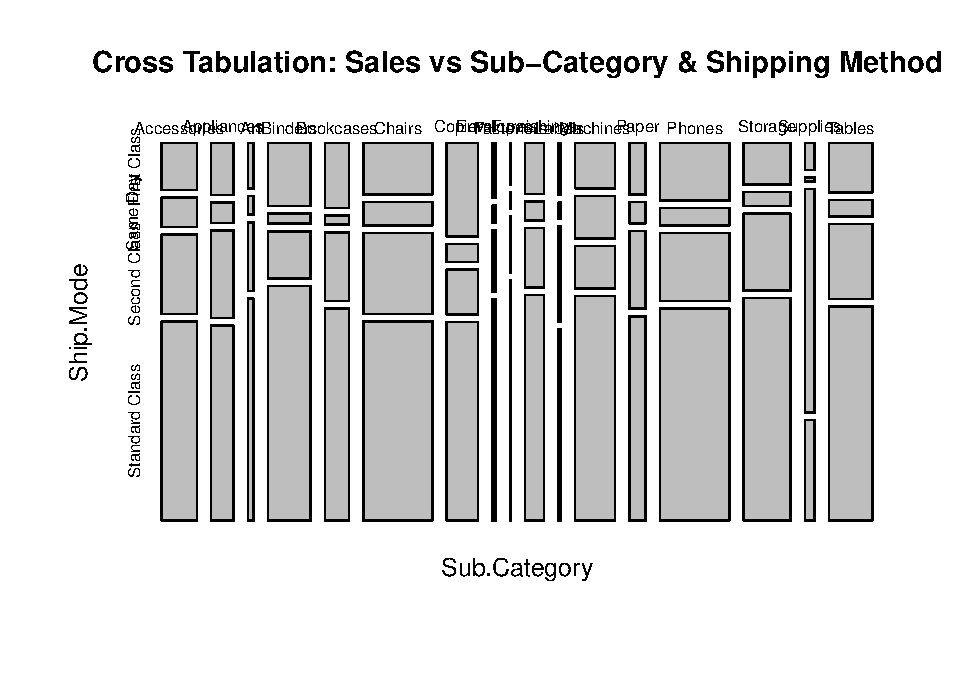
\includegraphics{p4ds_files/figure-latex/unnamed-chunk-47-1} \end{center}

Another way to visualize the cross-tabulation above is through the use
of heatmap. In R a heatmap is created using the \texttt{heatmap}
function, so all we need to do is to swap the \texttt{plot()} function
above with \texttt{heatmap()}. I'd also set the heatmap to scale in the
column direction - this makes the heatmap output more sensible:

\begin{Shaded}
\begin{Highlighting}[]
\KeywordTok{heatmap}\NormalTok{(}\KeywordTok{xtabs}\NormalTok{(Sales }\OperatorTok{~}\StringTok{ }\NormalTok{Sub.Category }\OperatorTok{+}\StringTok{ }\NormalTok{Ship.Mode, retail), }\DataTypeTok{Colv =} \OtherTok{NA}\NormalTok{, }\DataTypeTok{Rowv =} \OtherTok{NA}\NormalTok{, }\DataTypeTok{cexCol =} \FloatTok{0.6}\NormalTok{,}\DataTypeTok{scale =} \StringTok{"column"}\NormalTok{)}
\end{Highlighting}
\end{Shaded}

\begin{center}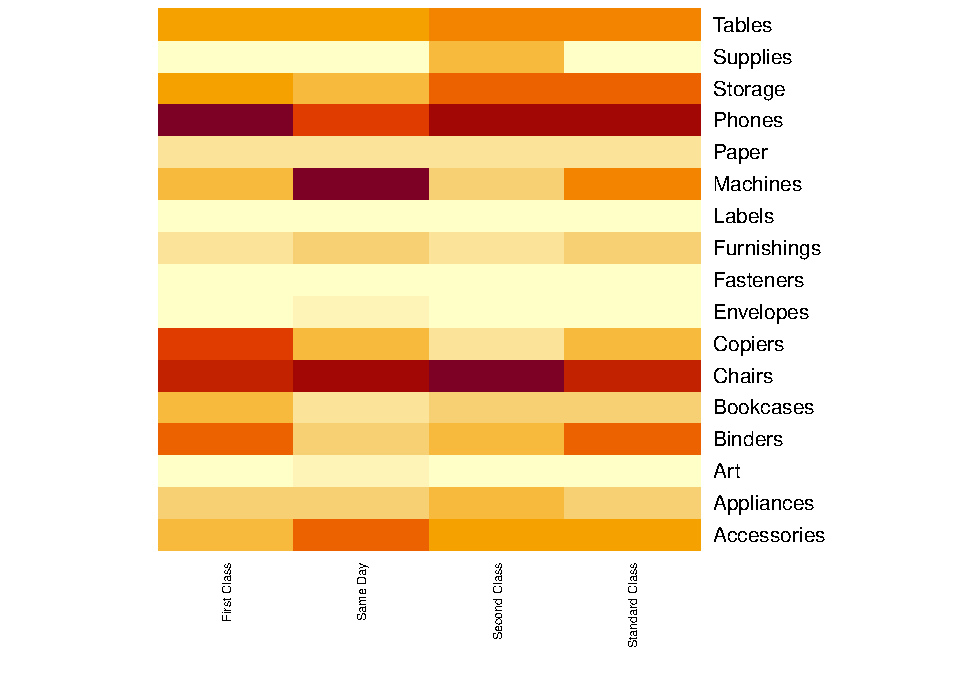
\includegraphics{p4ds_files/figure-latex/unnamed-chunk-48-1} \end{center}

Just like how there's more than one way to create a visual
representation of our cross-tabulation data, there are also more than
one way to summarize data across multiple variables. We've learned about
cross-tabulation using \texttt{xtabs} earlier but another equally common
statistical tool is the aggregate function, using \texttt{aggregate}.
The function call is almost the same as \texttt{xtabs} except is
requires an additional parameter, which is the function we want to use
for the aggregation:

\begin{Shaded}
\begin{Highlighting}[]
\KeywordTok{aggregate}\NormalTok{(Sales }\OperatorTok{~}\StringTok{ }\NormalTok{Category }\OperatorTok{+}\StringTok{ }\NormalTok{Sub.Category, retail, sum)}
\end{Highlighting}
\end{Shaded}

\begin{verbatim}
#>           Category Sub.Category     Sales
#> 1       Technology  Accessories 167380.32
#> 2  Office Supplies   Appliances 107532.16
#> 3  Office Supplies          Art  27118.79
#> 4  Office Supplies      Binders 203412.73
#> 5        Furniture    Bookcases 114880.00
#> 6        Furniture       Chairs 328449.10
#> 7       Technology      Copiers 149528.03
#> 8  Office Supplies    Envelopes  16476.40
#> 9  Office Supplies    Fasteners   3024.28
#> 10       Furniture  Furnishings  91705.16
#> 11 Office Supplies       Labels  12486.31
#> 12      Technology     Machines 189238.63
#> 13 Office Supplies        Paper  78479.21
#> 14      Technology       Phones 330007.05
#> 15 Office Supplies      Storage 223843.61
#> 16 Office Supplies     Supplies  46673.54
#> 17       Furniture       Tables 206965.53
\end{verbatim}

Compare that to the first few rows of results we obtained from
\texttt{xtabs()}:

\begin{Shaded}
\begin{Highlighting}[]
\KeywordTok{head}\NormalTok{(}\KeywordTok{xtabs}\NormalTok{(Sales }\OperatorTok{~}\StringTok{ }\NormalTok{Sub.Category }\OperatorTok{+}\StringTok{ }\NormalTok{Category, retail))}
\end{Highlighting}
\end{Shaded}

\begin{verbatim}
#>              Category
#> Sub.Category  Furniture Office Supplies Technology
#>   Accessories      0.00            0.00  167380.32
#>   Appliances       0.00       107532.16       0.00
#>   Art              0.00        27118.79       0.00
#>   Binders          0.00       203412.73       0.00
#>   Bookcases   114880.00            0.00       0.00
#>   Chairs      328449.10            0.00       0.00
\end{verbatim}

\textbf{Dive Deeper: Analyzing profitability by Category and Shipment
Mode}

Supposed you were assigned by the company to identify the type of
transactions that result in the highest profit on average as well as the
ones that result in the biggest losses (or lowest profit) per
transaction, how would you go about it?

Use the \texttt{aggregate()} function with \texttt{Sub.Category} and
\texttt{Ship.Mode}, but replace the \texttt{sum} with \texttt{mean} so
the function finds the ``average'' profit instead of total profit from
each group instead. If you did this correctly, you should observe that
Copiers are great profit makers, and that customers that ship Copiers on
First Class bags an average profit in excess of \$1,200 per transaction.
Sweet!

\begin{itemize}
\tightlist
\item
  What are the top 6 groups measured by average profit? Use the
  \texttt{mean} for this.\\
\item
  What the bottom (worst) 6 groups measured by average profit? Use the
  \texttt{mean} for this.\\
\item
  Use the answer provided at the end of this course book as reference.
\end{itemize}

Supposed we have no concern about the average transaction nor the
shipment mode, we could change the formula in our \texttt{aggregate}
function to take a much simpler form. The following code sums profit
across each sub-category:

\begin{Shaded}
\begin{Highlighting}[]
\KeywordTok{aggregate}\NormalTok{(Profit }\OperatorTok{~}\StringTok{ }\NormalTok{Sub.Category, retail, sum)}
\end{Highlighting}
\end{Shaded}

\begin{verbatim}
#>    Sub.Category      Profit
#> 1   Accessories  41936.6357
#> 2    Appliances  18138.0054
#> 3           Art   6527.7870
#> 4       Binders  30221.7633
#> 5     Bookcases  -3472.5560
#> 6        Chairs  26590.1663
#> 7       Copiers  55617.8249
#> 8     Envelopes   6964.1767
#> 9     Fasteners    949.5182
#> 10  Furnishings  13059.1436
#> 11       Labels   5546.2540
#> 12     Machines   3384.7569
#> 13        Paper  34053.5693
#> 14       Phones  44515.7306
#> 15      Storage  21278.8264
#> 16     Supplies  -1189.0995
#> 17       Tables -17725.4811
\end{verbatim}

And we can confirm the above by summing across the row values in our
\texttt{xtabs} as well, using a handy function called \texttt{rowSums}:

\begin{Shaded}
\begin{Highlighting}[]
\KeywordTok{as.data.frame}\NormalTok{(}\KeywordTok{rowSums}\NormalTok{(}\KeywordTok{xtabs}\NormalTok{(Profit }\OperatorTok{~}\StringTok{ }\NormalTok{Sub.Category }\OperatorTok{+}\StringTok{ }\NormalTok{Ship.Mode, retail)))}
\end{Highlighting}
\end{Shaded}

\begin{verbatim}
#>             rowSums(xtabs(Profit ~ Sub.Category + Ship.Mode, retail))
#> Accessories                                                41936.6357
#> Appliances                                                 18138.0054
#> Art                                                         6527.7870
#> Binders                                                    30221.7633
#> Bookcases                                                  -3472.5560
#> Chairs                                                     26590.1663
#> Copiers                                                    55617.8249
#> Envelopes                                                   6964.1767
#> Fasteners                                                    949.5182
#> Furnishings                                                13059.1436
#> Labels                                                      5546.2540
#> Machines                                                    3384.7569
#> Paper                                                      34053.5693
#> Phones                                                     44515.7306
#> Storage                                                    21278.8264
#> Supplies                                                   -1189.0995
#> Tables                                                    -17725.4811
\end{verbatim}

\hypertarget{r-scripts-and-reproducible-research}{%
\section{R Scripts and Reproducible
Research}\label{r-scripts-and-reproducible-research}}

If you are new to writing code but you've scored at least 2 of the 3
quizzes in this coursebook - congratulations! We'll now finish strongly
by attempting one of the two learn-by-building modules. As this is a
graded task for our Academy students, completion of the task is not
optional and count towards your final score. You can choose to complete
either of the following task:

\textbf{R Script to clean \& transform the data}\\
Write a R script containing a function (name the function however way
you want) that reads \texttt{retail.csv} as input, perform the necessary
transformation and export a cross-tabulation numeric result OR plot as
output. This is the base requirement but more advanced students are free
to customize their script to add any extra functionalities.

\begin{Shaded}
\begin{Highlighting}[]
\CommentTok{# Sourcing the scipt and running the function should print a cross-tabulation result or plot}
\KeywordTok{source}\NormalTok{(}\StringTok{"lbb1.R"}\NormalTok{)}
\KeywordTok{crstab}\NormalTok{()}
\end{Highlighting}
\end{Shaded}

For graders: Student scores a maximum 2 out of (2) possible points.
Check that the R script executes and return a cross tabulation plot
(\texttt{plot(xtabs())}) with no errors, warnings or missing variables /
values.

\textbf{Reproducible Data Science}\\
Create an R Markdown file that combines your step-by-step data
transformation code with some explanatory text. Add formatting styles
and hierarchical structure using Markdown.

For graders: Student scores a maximum 2 out of (2) possible points.
Check that the RMD file compiles to HTML with at least \textbf{two}
headings, \textbf{two} explanatory paragraph, and the final output is a
business recommendation written in English or Bahasa Indonesia on
profitable categories.

Writing your code as R scripts make all of these metrics possible for
further automation and integration with other tools and services, while
writing a R Markdown presents your findings and recommendations in a way
that is friendly to non-technical / managerial team members.

\hypertarget{tips-on-writing-r-scripts-and-functions}{%
\subsection{Tips on writing R Scripts and
functions}\label{tips-on-writing-r-scripts-and-functions}}

As an example, here's how you can write a function, named
``weeklyreport'':

\begin{Shaded}
\begin{Highlighting}[]
\KeywordTok{library}\NormalTok{(skimr)}
\KeywordTok{library}\NormalTok{(dplyr)}
\NormalTok{weeklyreport <-}\StringTok{ }\ControlFlowTok{function}\NormalTok{()\{}
\NormalTok{  retail <-}\StringTok{ }\KeywordTok{read.csv}\NormalTok{(}\StringTok{"data_input/retail.csv"}\NormalTok{) }\OperatorTok\StringTok{ }
\StringTok{  }\KeywordTok{group_by}\NormalTok{(Segment) }\OperatorTok\StringTok{ }
\StringTok{  }\KeywordTok{skim}\NormalTok{(Category, Profit)}
\NormalTok{\}}
\end{Highlighting}
\end{Shaded}

And now you can call the function you created:

\begin{Shaded}
\begin{Highlighting}[]
\KeywordTok{weeklyreport}\NormalTok{()}
\end{Highlighting}
\end{Shaded}

\hypertarget{annotations}{%
\section{Annotations}\label{annotations}}

\end{document}
